\section{Durchführung}
\label{sec:Durchführung}

Bei diesem Experiment wird als Lichtquelle ein He-Ne-Laser mit Wellenlänge $\lambda = \SI{635}{\nano\metre}$ verwendet.
Dieser befindet sich in Deckung mit dem zu untersuchenden Spalt und dem verschiebbaren Photoelement.
Die Spalte werden kurz hinter dem Laser in einer Vorrichtung befestigt.
Es wird ein fester Einzelspalt und zwei unterschiedliche Doppelspalte untersucht.
Das Photoelement befindet sich in einigem Abstand hinter dem Spalt.
Es ist auf einer verschiebbaren Plattform angebracht.
Diese kann auf $\SI{10}{\micro\metre}$ genau eingestellt werden.
Dies geschieht durch Drehen einer Trommel, welche an dem Messverschiebereiter befestigt ist.
Das Photoelement ist mit einem Amperemeter verbunden, welches die Messung des Stroms in Abhängigkeit von der Intensitätsverteilung des durch den Spalt gebeugten Lichtes ermöglicht.
Der generelle Aufbau ist in Abbildung \ref{fig:Aufbau} dargestellt.

\begin{figure}
  \centering
  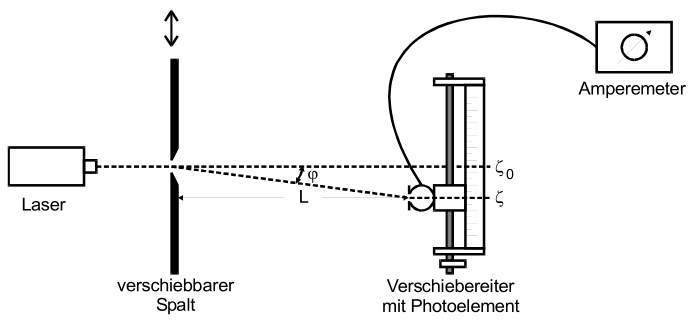
\includegraphics[scale=0.7]{images/Aufbau.png}
  \caption{Der generelle Versuchsaufbau, entnommen der Versuchsanleitung \cite[36]{1}}
  \label{fig:Aufbau}
\end{figure}

Für die eigentliche Messung wird der Spalt in der entsprechenden Vorrichtung fixiert.
Um eine optimale Intensitätsverteilung zu gewährleisten, wird das Beugungsbild zunächst an einer Abschirmung abgefangen und der Spalt dann so verschoben, dass die Verteilung gut erkennbar ist.
In diesem Zuge wird auch der Dunkelstrom $I_D$ gemessen.
Die Abschirmung wird entfernt und der Strom in Abhängigkeit von der Postion des Verschiebereiters gemessen.
Dafür wird das Beugungsbild in geeigneten Teilschritten abgefahren.
Bei dem Einzelspalt werden die ersten Nebenmaxima mitgemessen, bei den Doppelspalten die zweiten.
In der Nähe der größten Veränderung sollte am genauesten gemessen werden.
